\section{Objects, classes, messages, arguments}

SuperCollider is an Object-Oriented programming language, like Java or C++. It is beyond the scope of this tutorial to explain what this means, so we'll let you search that on the web if you are curious. Here we'll just explain a few basic concepts you need to know to better understand this new language you are learning.

Everything in SuperCollider is an \emph{object}. Even simple numbers are objects in SC. Different objects behave in different ways and hold different kinds of information. You can request some info or action from an object by sending it a \emph{message}. When you write something like \texttt{2.squared}, the message \texttt{squared} is being sent to the receiver object \texttt{2}. The dot between them makes the connection. Messages are also called \emph{methods}, by the way.

Objects are specified hierarchically in \emph{classes}. SuperCollider comes with a huge collection of pre-defined classes, each with their own set of methods.

Here's a good way to understand this. Let's imagine there is an abstract class of objects called \texttt{Animal}. The Animal class defines a few general methods (messages) common to all animals. Methods like \texttt{age}, \texttt{weight}, \texttt{picture} could be used to get information about the animal. Methods like \texttt{move}, \texttt{eat}, \texttt{sleep} would make the animal perform a specific action. Then we could have two subclasses of Animal: one called \texttt{Pet}, another called \texttt{Wild}. Each one of these subclasses could have even more subclasses derived from them (like \texttt{Dog} and \texttt{Cat} derived from \texttt{Pet}). Subclasses inherit all methods from their parent classes, and implement new methods of their own to add specialized features. For example, both Dog and Cat objects would happily respond to the \texttt{.eat} message, inherited from the Animal class. \texttt{Dog.name} and \texttt{Cat.name} would return the name of the pet: this method is common to all objects derived from Pet.  \texttt{Dog} has a \texttt{bark} method, so you can call \texttt{Dog.bark} and it will know what to do. \texttt{Cat.bark} would throw you an error message: \texttt{ERROR: Message 'bark' not understood.}

In all these hypothetical examples, the words beginning with a capital letter are \emph{classes} which represent \emph{objects}. The lowercase words after the dot are \emph{messages} (or \emph{methods}) being sent to those objects. Sending a message to an object always returns some kind of information. Finally, messages sometimes accept (or even require) \emph{arguments}. Arguments are the things that come inside parentheses right after a message. In \texttt{Cat.eat("sardines", 2)}, the message \texttt{eat} is being sent to \texttt{Cat} with some very specific information: what to eat, and quantity. Sometimes you will see arguments declared explicitly inside the parentheses (keywords ending with a colon). This is often handy to remind the reader what the argument refers to. \texttt{Dog.bark(volume: 10)} is more self-explanatory than just \texttt{Dog.bark(10)}.

\begin{figure}[h]
\centerline{\framebox{
	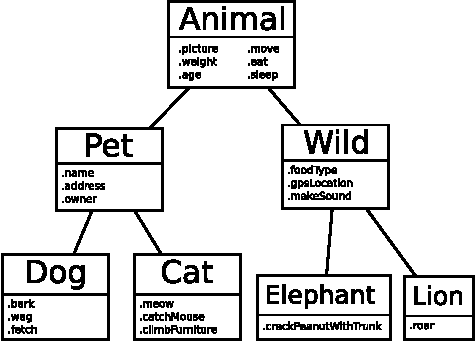
\includegraphics[scale=0.9]{fig-animal-class-chart.pdf}}}
\caption{Hypothetical class hierarchy.}
\label{fig:animal-class-chart}
\end{figure}

OK---enough of this quick and dirty explanation of object-oriented programming. Let's try some examples that you can actually run in SuperCollider. Run one line after the other and see if you can identify the message, the receiver object, and the arguments (if any). The basic structure is \texttt{Receiver.message(arguments)} Answers at the end of this document.\endnote{First line: the Array \texttt{[1, 2, 3, "wow"]} is the receiving object; \texttt{reverse} is the message. Second line: the String "hello" is the receiving object; \texttt{dup} is the message; \texttt{4} is the argument to \texttt{dup}. Third line: 3.1415 is the receiving object; \texttt{round} is the message; \texttt{0.1} is the argument to \texttt{round}. Fourth line: \texttt{100} is the receiver object, \texttt{rand} is the message. Last line: \texttt{100.0} is the receiver of the message \texttt{rand}, the result of which is a random number between 0 and 100. That number becomes the receiver of the message \texttt{round} with argument \texttt{0.01}, so that the random number is rounded to two decimal cases. Then this result becomes the receiving object of the message \texttt{dup} with argument \texttt{4}, which creates a list with four duplicates of that number.}

 
\begin{lstlisting}[style=SuperCollider-IDE, basicstyle=\scttfamily\footnotesize]
[1, 2, 3, "wow"].reverse;
"hello".dup(4); 
3.1415.round(0.1); // note that the first dot is the decimal case of 3.1415
100.rand; // evaluate this line several times
// Chaining messages is fun:
100.0.rand.round(0.01).dup(4);
\end{lstlisting}